Tässä kappaleessa käsitellään uutta kaatosysteemiä, jonka avulla pyritään ratkaisemaan edellisessä kappaleessa käsiteltyjä ongelmia. Se sisältää sekä logiikan että robottikoodin, sekä näiden kahden rajapinnan.

% Lisää tietoa LogicLayerin toiminnasta tähän tai kpl 2.1?

Logiikkakerros kutsuu logiikan funktiota PourBottle, joka käsittelee kaatoa yksittäisestä pullosta. Nyt uutena logiikkaan on toteutettu funktio HandlePour. Tämä kutsuu vaakaa ja käskee robottia lopettamaan kaadon, kun vaa'an lukema on tarpeeksi suuri.

\begin{figure}[h]
\begin{center}
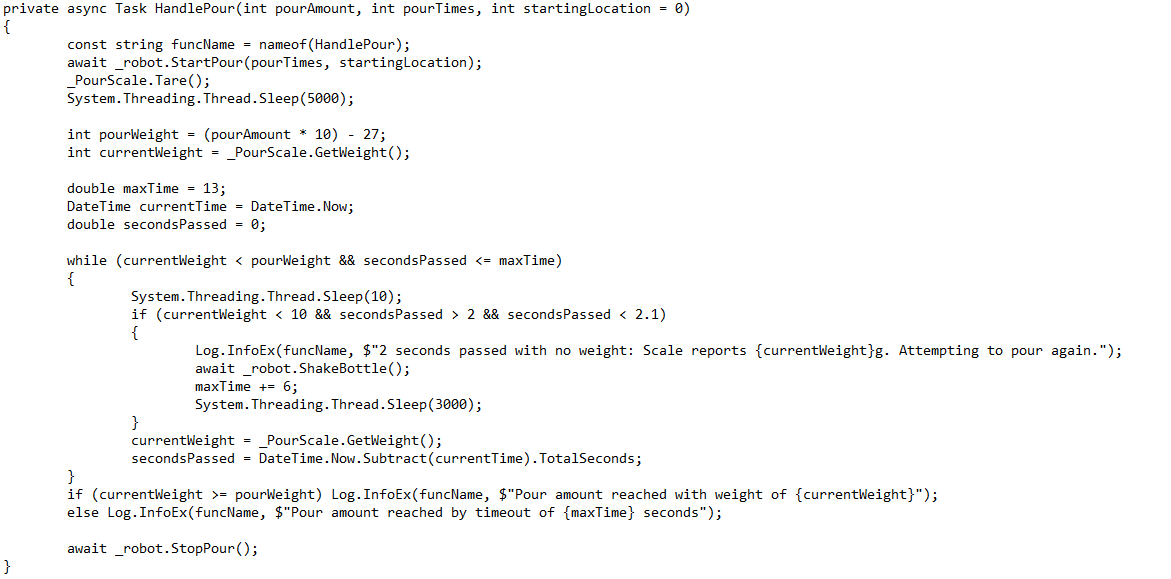
\includegraphics[scale=0.6]{img/HandlePour.png}
\end{center}
\caption{HandlePour-funktio}
\label{fig:HandlePour}
\end{figure}

HandlePour kutsuu ensin RobotCellLayerin funktiota StartPour. RobotCellLayer vastaa robotin kanssa kommunikoinnista. StartPour kutsuu robotin jobia, joka on tällä hetkellä nimellä NEWPOUR.

\begin{figure}[h]
\begin{center}
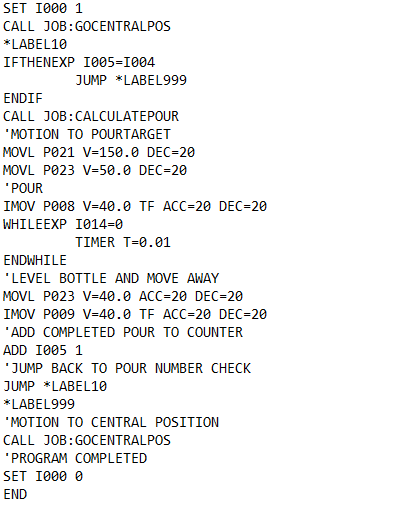
\includegraphics[scale=0.8]{img/NEWPOUR.png}
\end{center}
\caption{NEWPOUR-robottijobi}
\label{fig:NEWPOUR}
\end{figure}
\newpage

NEWPOUR-job on robotin liikkeiltään hyvin samantapainen kuin kappaleessa \ref{ch:vanha_kaato} esitetty POURDRINKS. Se robottia siirtymään kaatopisteelle ja kallistaa pulloa aloittaen kaadon. Uutta on kuitenkin se, että robotti jää while-loopin ansiosta odottamaan, että muuttuja I014 on 0.

HandlePour-funktio laskee halutun painon kertomalla halutun nesteen tilavuuden, joka on senttilitroina, kymmenellä, jolloin saadaan haluttu massa grammoina.
